% ============================================================
% Ejercicio 1
% ============================================================
\section{Ejercicio 1}

\begin{tcolorbox}[enunciado]
Sean $L_{1}$, $L_{2}$ definidos sobre $\Sigma^{*}$. Definimos la operación $\oplus$ de la siguiente manera:

\[ L_{1} \oplus L_{2} = \{x \mid x \text{ está en exactamente uno de los lenguajes, en } L_{1} \text{ o (exclusivo) en } L_{2}\} \]

Supón que ambos lenguajes, $L_{1}$, $L_{2}$, pertenecen a las clases de complejidad NP y coNP. 

Prueba que $L_{1} \oplus L_{2} \in \text{NP} \cap \text{coNP}$.
\end{tcolorbox}

\subsection*{Solución}
\begin{figure}[H]
    \centering
    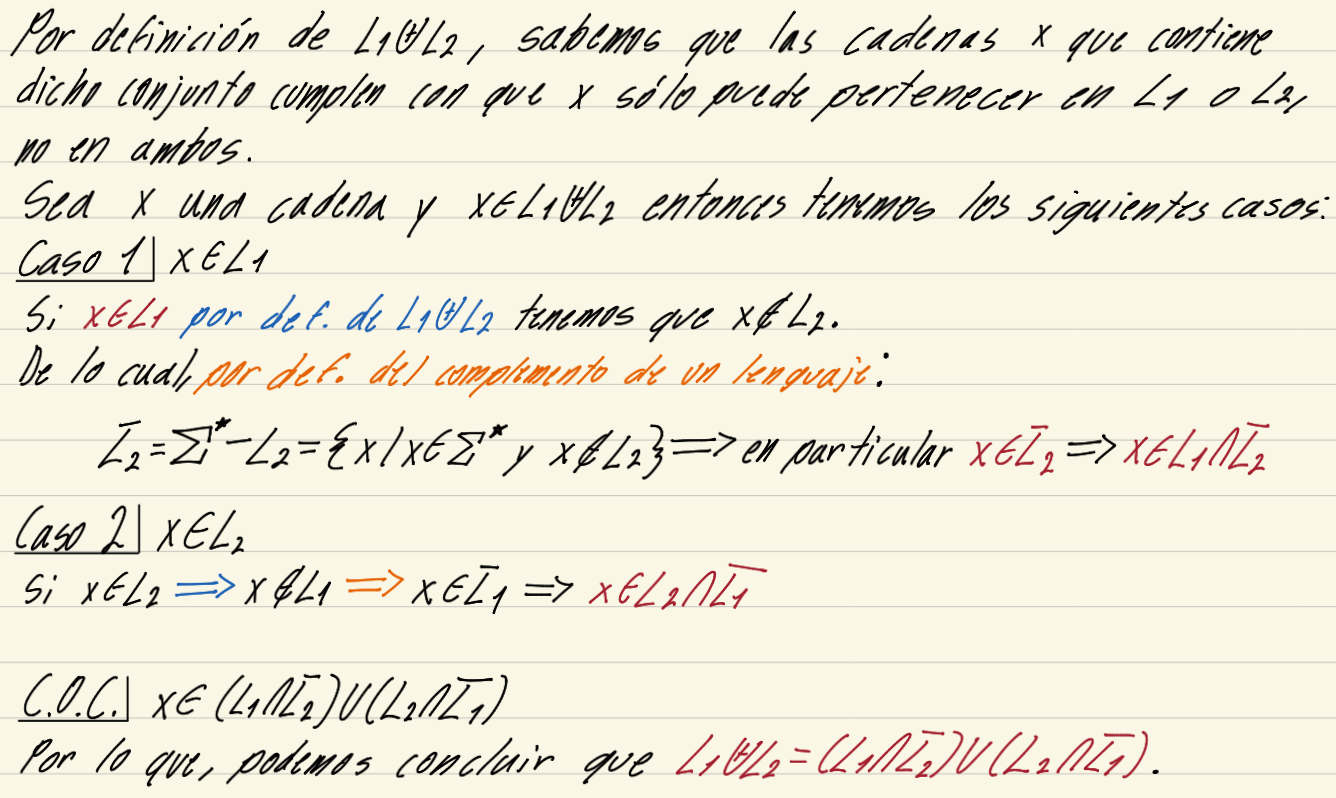
\includegraphics[width=0.8\linewidth]{imagenes/01_ejercicio/01_image.png}
\end{figure}

\begin{figure}[H]
    \centering
    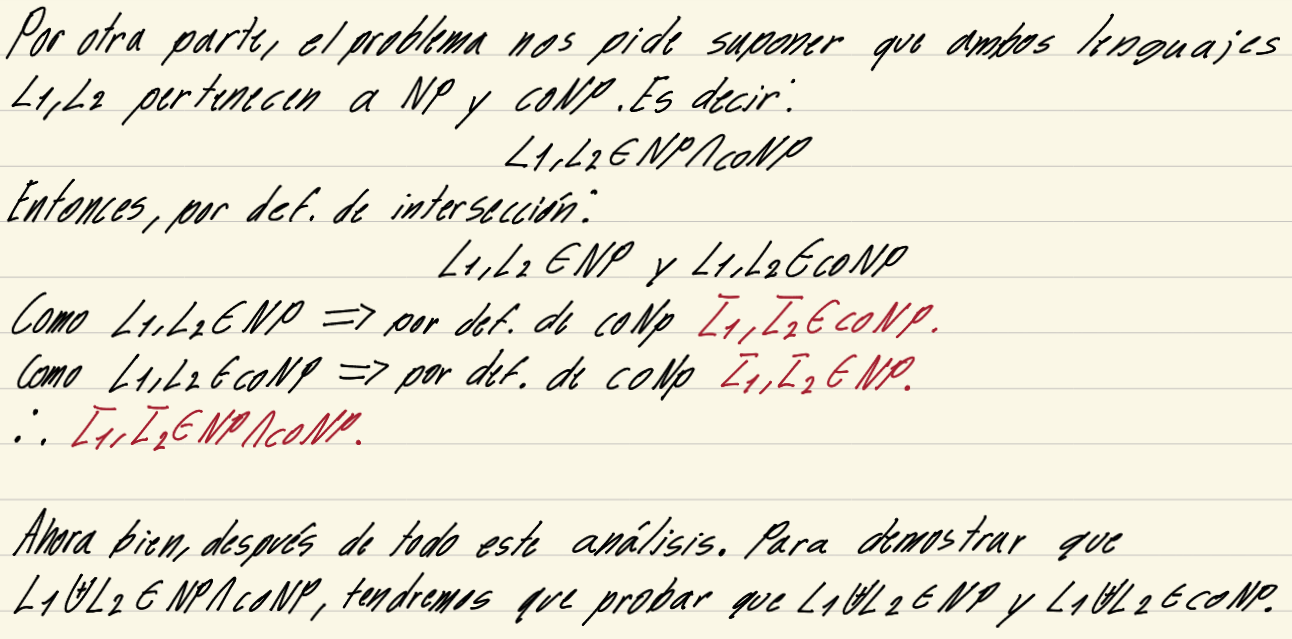
\includegraphics[width=0.8\linewidth]{imagenes/01_ejercicio/02_image.png}
\end{figure}

\begin{figure}[H]
    \centering
    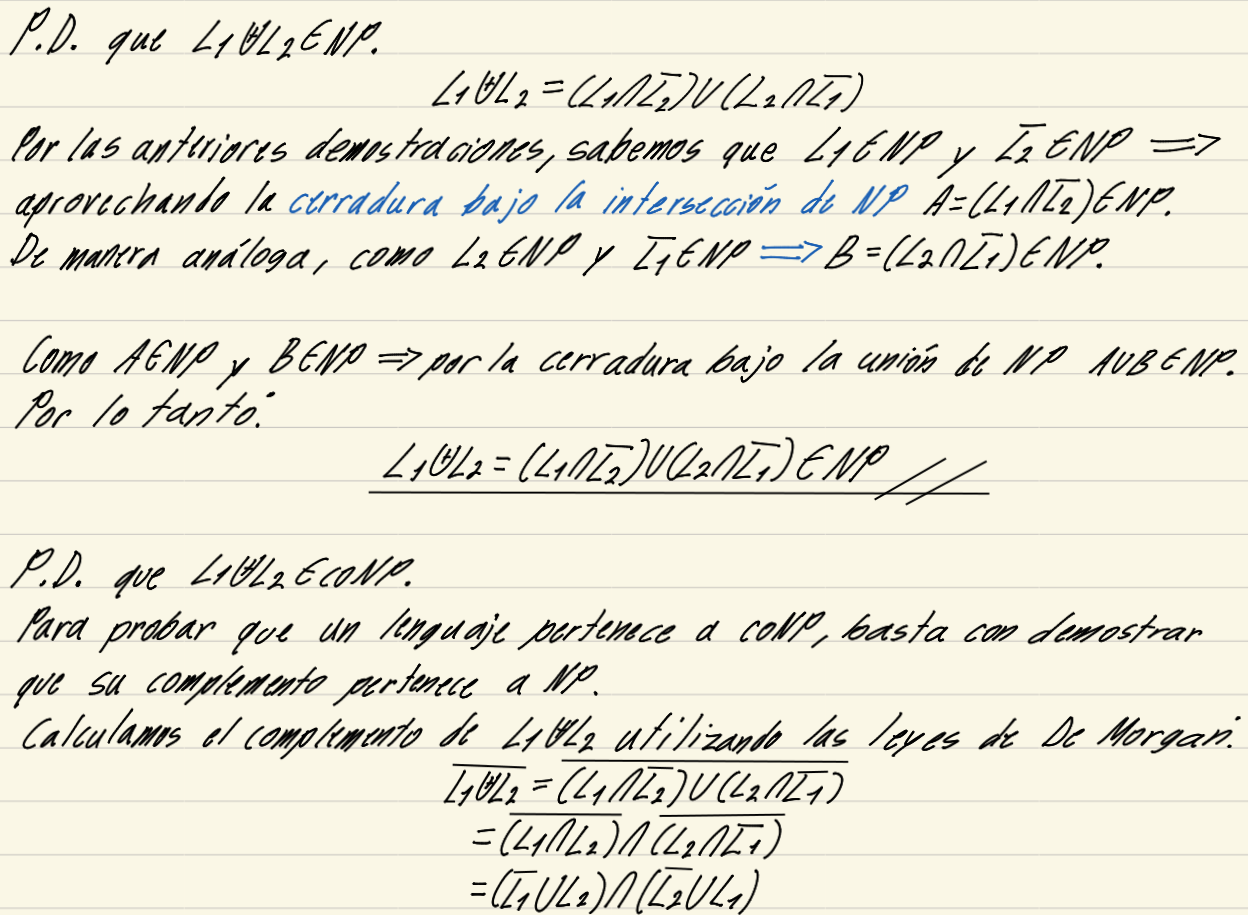
\includegraphics[width=0.8\linewidth]{imagenes/01_ejercicio/03_image.png}
\end{figure}

\begin{figure}[H]
    \centering
    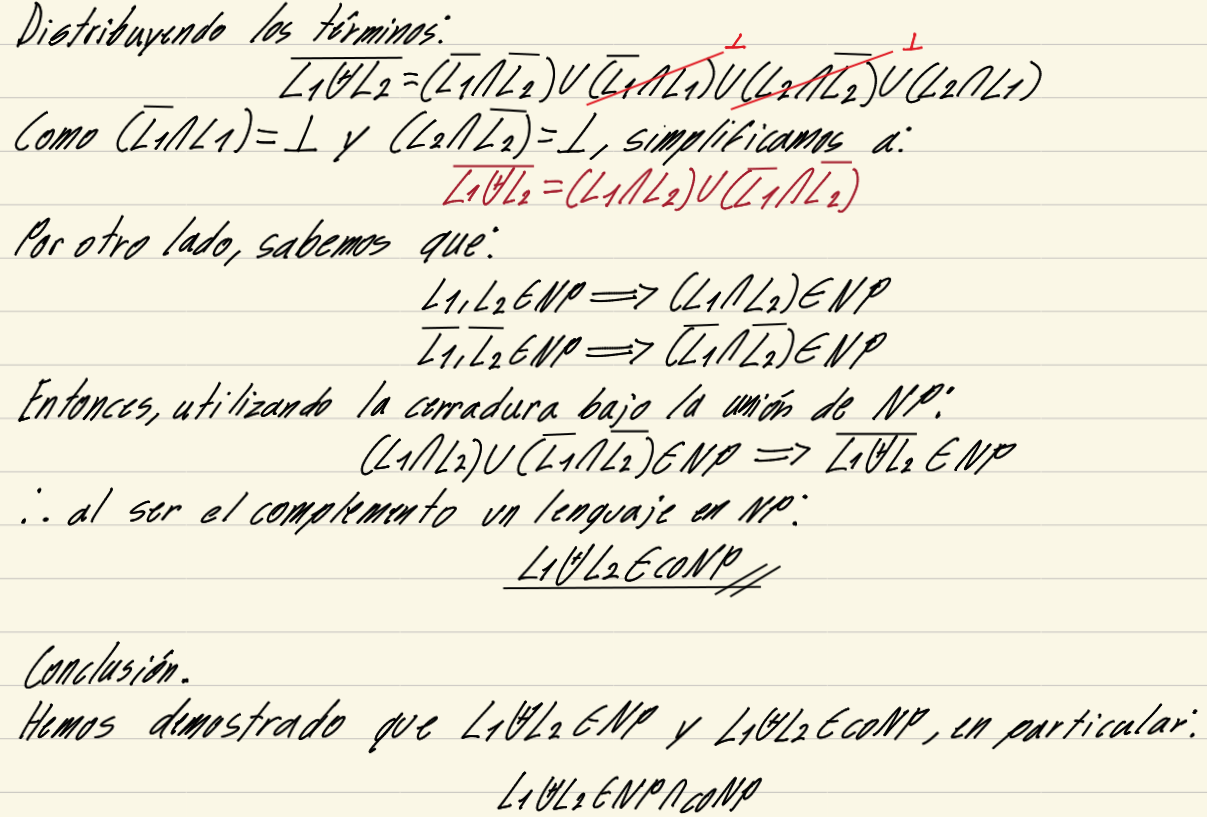
\includegraphics[width=0.8\linewidth]{imagenes/01_ejercicio/04_image.png}
\end{figure}